\pdfbookmark{Общая характеристика работы}{characteristic}             % Закладка pdf
\section*{Общая характеристика работы}

\newcommand{\actuality}{\pdfbookmark[1]{Актуальность}{actuality}\underline{\textbf{\actualityTXT}}}
\newcommand{\progress}{\pdfbookmark[1]{Разработанность темы}{progress}\underline{\textbf{\progressTXT}}}

\newcommand{\objectresearch}{\pdfbookmark[1]{Объект исследования}{progress}\underline{\textbf{\objectresearchTXT}}}

\newcommand{\subjectresearch}{\pdfbookmark[1]{Предмет исследования}{progress}\underline{\textbf{\subjectresearchTXT}}}

\newcommand{\aim}{\pdfbookmark[1]{Цели}{aim}\underline{{\textbf\aimTXT}}}
\newcommand{\tasks}{\pdfbookmark[1]{Задачи}{tasks}\underline{\textbf{\tasksTXT}}}
\newcommand{\aimtasks}{\pdfbookmark[1]{Цели и задачи}{aimtasks}\aimtasksTXT}
\newcommand{\novelty}{\pdfbookmark[1]{Научная новизна}{novelty}\underline{\textbf{\noveltyTXT}}}
\newcommand{\influence}{\pdfbookmark[1]{Практическая значимость}{influence}\underline{\textbf{\influenceTXT}}}
\newcommand{\elaboration}{\pdfbookmark[1]{Степень разработанности темы}{elaboration}\underline{\textbf{\elaborationTXT}}}
\newcommand{\methods}{\pdfbookmark[1]{Методы исследования}{methods}\underline{\textbf{\methodsTXT}}}
\newcommand{\defpositions}{\pdfbookmark[1]{Положения, выносимые на защиту}{defpositions}\underline{\textbf{\defpositionsTXT}}}
\newcommand{\reliability}{\pdfbookmark[1]{Достоверность}{reliability}\underline{\textbf{\reliabilityTXT}}}
\newcommand{\probation}{\pdfbookmark[1]{Апробация}{probation}\underline{\textbf{\probationTXT}}}
\newcommand{\contribution}{\pdfbookmark[1]{Личный вклад}{contribution}\underline{\textbf{\contributionTXT}}}
\newcommand{\publications}{\pdfbookmark[1]{Публикации}{publications}\underline{\textbf{\publicationsTXT}}}

{\actuality} 

% В настоящее время заметна тенденция цифровой трансформации, что подразумевает под собой бурное развитие информационных технологий во всех сферах деятельности человека. Основными перспективными направлениями цифровизации, на которые сделан акцент в диссертационной работе, являются цифровая трансформация транспортного комплекса и глобальная цифровизация нефтегазового сектора страны. Этот подход подразумевает не только оснащение современным технологичным оборудованием, но и глобальное изменение в подходах управления, сбора информации и средств коммуникаций. Уже сейчас основными современными информационными технологиями, встречающимися на пути трансформации являются: большие данные (Big Data), предиктивные модели на искусственных нейронных сетях (Artificial Neural Network), системы распределенного реестра (Blockchain), промышленный интернет вещей (Industrial Internet of Things, IIoT), технологии виртуальной и дополненной реальности (Virtual Reality, VR), мониторинг распределенных объектов с помощью беспилотных летательных аппаратов БПЛА (Unmanned Aerial Vehicle, UAV). В совокупности данные технологии создают необходимость в эффективной передаче больших объемов высокоскоростного трафика. Одним из путей решенияй проблемы является интенсивное развитие и внедрение беспроводных технологий.

% \fixme{В настоящее время заметна тенденция бурного развития информационных технологий во всех сферах деятельности человека. На сегодня 

% оказывает весомое влияние на нефтегазовый сектор страны. Современные компании, представляющие собой сложные многоуровневые производственные системы, для своего устойчивого развития требуют постоянного развития и совершенствования передовых технологий.  Сегодня наблюдается  бурное развитие процесса «цифровизации» нефтегазовой отрасли. Крупные международные нефтегазовые компании имеют подразделения, задачами которых является разработка и реализация принципов интеллектуального месторождения \cite{Tcharo2018} на промысле, организация безопасности на технологических объектах, развитие концепции  перехода к малолюдным системам управления добычей, транспортировкой и переработкой сырья. Уже сейчас основными современными информационными технологиями, встречающиеся в отрасли являются: большие данные (Big Data), предикстивные модели на искусственных нейронных сетях (Artificial Neural Network), системы распределенного реестра (Blockchain), промышленный интернет вещей (Industrial internet of things, IIoT), технологии виртуальной и дополненной реальности (Virtual Reality, VR), мониторинг распределенных объектов с помощью беспилотных летательных аппаратов БПЛА (Unmanned Aerial Vehicle, UAV). }
 
 
% \fixme{В совокупности данные технологии создают необходимость эффективной передачи больших объемов высокоскоростного трафика. Информационные  системы современных  сегодня содержат колоссальный объем информации высокоскоростного мультимедийного трафика. Одним из путей решения является внедрение беспроводных технологий.}

Создание современной инфраструктуры передачи данных вдоль транспортных магистралей является одной из важнейших проблем при создании нового и функционировании существующего транспортного комплекса  \cite{Vishnevsky2016_Review_of_methodology}. Одним из путей решения проблемы является интенсивное развитие и внедрение беспроводных технологий. Активное использование беспроводных сетей основывается на ряде их преимуществ по сравнению с кабельными сетями:
\begin{itemize}
    \item организация связи в труднодоступных регионах;
    \item быстрый ввод в эксплуатацию по системе подключение типа <<Подключил и Работай>> (Plug-\&-Play);
    \item сокращение капитальных затрат на создание сети; 
    \item уменьшение затрат на эксплуатацию;
    \item высокая гибкость, мобильность, масштабируемость;
    \item упрощенные требования к обслуживанию оборудования.
\end{itemize}

В рамках этого процесса возникает актуальная научно-техническая проблема повышения качества топологического проектирования беспроводной сети связи, осуществляющей мониторинг, сбор и передачу информации в центр управления с множества объектов на заданной территории.   

% В совокупности со всеми вышеизложенными перспективными направлениями беспроводные технологии являются неотъемлемой частью «цифровизации» месторождения. Отсюда возникает научно - техническая проблема организации распределенной беспроводной сети связи, соответствующая реальным требованием современного производства.

% Большой объем передачи информации  привел к еще одной из наиболее интересных тенденций цифрового развития – внедрения беспроводных технологий. Современные месторождения сегодня, помимо данных первичного сбора и обработки информации технологических параметров основных производственных объектов содержат также колоссальный объем  информации мультимедийного трафика. Сюда входят данные БПЛА по обнаружению утечек и  разрушения трубопроводов; камер видеонаблюдений; а также большой поток данных цифровых двойников, аналитики и т.д. В совокупности со всеми вышеизложенными перспективными направлениями беспроводные технологии являются неотъемлемой частью «цифровизации» месторождения.



% Процесс проектирования современной  беспроводной сети связи состоит из последовательного решения взаимосвязанных задач:

% \begin{enumerate}
%     \item обследование местности;
%     \item выбор типов технических средств и протоколов;
%     \item выбор топологической структуры сети;
%     \item анализ и оценка будущей беспроводной сети с помощью математического моделирования.
% \end{enumerate}

Диссертация посвящена актуальной проблеме синтеза топологической структуры беспроводной широкополосной сети. Задача выбора топологической структуры при проектировании является одной из важнейших задач, ошибки при которой могут привести к большим капитальным затратам и ухудшению качества обслуживания (Quality Of Service, QoS). С математической точки зрения задача синтеза топологии является сложной задачей, время счета для которой растет экспоненциально с ростом размерности. Таким образом, высокий теоретический и практический интерес к разработке новых моделей и методов оптимизации топологической структуры беспроводной широкополосной сети определяет актуальность и новизну диссертационной работы.


% Задача синтеза топологии при комплексном проектировании БШС является основной проблемой исследования в данной работе.

% В.М. Вишневский, Ю. В. Гайдамака, А.Е. Кучерявый, А.А. Ларионов, В.М. Малыш,  О.Ю. Першин, К. Е. Самуйлов, Р.Л. Смелянский и другие.

% Создание и постоянное развитие современной инфраструктуры передачи данных является одной из основных задач цифровизации. Бурное развитие беспроводных сетей во всех областях деятельности человека: интеллектуальные транспортные системы вдоль автомобильных дорог, мониторинг нефтегазовых объектов, организация современного высокоскоростного покрытия в общественных зонах обосновывают целесообразность их использования. 

% и, в частности, решающие задачу синтеза топологии В. М. Вишневский, А. А. Ларионов, В.М. Малыш, О. Ю. Першин.

{\progress} В настоящее время в России и за рубежом исследованию беспроводных сетей связи посвящен ряд работ, где рассматриваются сети для мониторинга гражданских  и промышленных объектов. Примерами таких объектов является жилые районы города, протяженные автомагистрали, линии метрополитена и железные дороги, магистральные трубопроводы и др. При исследовании проблемы синтеза топологии сети автор опирался на труды отечественных ученых, занимающихся исследованиями в области телекоммуникационных сетей: В.М. Вишневский, Ю. В. Гайдамака, Р.В. Киричек, А. Е. Кучерявый, Е. А. Кучерявый, А. А. Ларионов, В. М. Малыш,  О. Ю. Першин, К. Е. Самуйлов, Р. Л. Смелянский. Наряду с отечественными работами указанные проблемы рассматривались в работах зарубежных авторов: Е.С. Кавальканте, Х. Лиу, А.Б. Рейз, Д.Ли, Д.П. Хейман, С. Шен, Д. Бендель, У. М. Амин, Б. Брахим, Х.Э. Кызылёз и др. В работах указанных авторов рассматриваются задачи оптимального синтеза топологии сети и исследуются вопросы анализа сетей, в том числе рассматриваются оценки характеристик сетей с помощью стохастических моделей сетей массового обслуживания. 

В диссертации представлены новые математические модели задачи оптимального размещения базовых станций беспроводной широкополосной сети, предложен новый алгоритм типа ветвей и границ для решения задачи в комбинаторной форме.
Исследования доведены до разработки алгоритмов и комплексов программ, применимых для решения практических задач. Приведены результаты численных экспериментов, позволяющие оценить характеристики вычислительных методов.


{\objectresearch} являются сети специальных типов, широко представленных на практике: беспроводные широкополосные сети вдоль протяженных транспортных магистралей и беспроводные широкополосные сети с ячеистой топологией (mesh) для телекоммуникационного покрытия объектов, рассредоточенных на заданной территории.

% являются беспроводные широкополосные сети вдоль протяженных транспортных магистралей: автомобильные и железные дороги, магистральные и промысловые трубопроводы, линии метрополитена. 

% специальных типов, широко представленных на практике: БШС для контроля линейного участка и БШС с ячеистой топологией (mesh) для контроля объектов, рассредоточенных на заданной территории.

{\subjectresearch} является синтез топологической структуры беспроводной широкополосной сети.

{\aim} состоит в разработке моделей и методов оптимального размещения базовых станций для беспроводных широкополосных сетей, определяющих топологию таких сетей.

Для достижения поставленной цели были решены следующие {\tasks}:
\begin{enumerate}[beginpenalty=10000] % https://tex.stackexchange.com/a/476052/104425
  \item Проведен анализ современного состояния и перспектив развития беспроводных широкополосных сетей для обоснования  актуальности и новизны исследований в области оптимизации их топологии. 
  \item Проанализирована методика проектирования современных беспроводных широкополосных сетей с целью определения требований к решению задачи синтеза оптимальной топологии сети, а также расчета параметров беспроводной сети, необходимых для решения задач размещения базовых станций.
  \item Сформулированы математические модели для задачи оптимального размещения базовых станций беспроводной широкополосной сети с линейной топологией, разработан алгоритм типа ветвей и границ для решения указанной задачи, предложена итерационная процедура нахождения последовательности лучших решений в размещении базовых станций в рамках комплексного проектирования сети.
  \item Сформулирована математическая модель в виде задачи частично целочисленного линейного программирования для решения задач проектирования и анализа беспроводных широкополосных сетей с ячеистой топологией.
%   \item Разработан программный комплекс для расчета задачи размещения оптимального размещения базовых станций.
  \item Приведены численные эксперименты, доказывающие значимость представленных математических моделей и разработанного алгоритма.
  %   \item разработаны методы оценки характеристик производительности сети с помощью данных имитационного моделирования и методов машинного обучения. 

\end{enumerate}

 

{\novelty} результатов исследования заключается в следующем:
\begin{enumerate}[beginpenalty=10000] % https://tex.stackexchange.com/a/476052/104425

    \item Разработана новая математическая модель целочисленного линейного программирования задачи оптимального размещения базовых станций при проектировании беспроводной широкополосной сети с линейной топологией. 
    \item Разработан специальный алгоритм типа ветвей и границ для численного решения задачи в виде комбинаторной модели в экстремальной форме, учитывающей специфику размещения базовых станций беспроводной широкополосной сети для телекоммуникационного покрытия протяженных объектов. 
    % \item Разработана новая комбинаторная модель в экстремальной форме решения задачи оптимального размещения базовых станций при проектировании БШС с линейной топологией.   
    % \item Разработан специальный алгоритм типа ветвей и границ для решения численным методом сформулированной экстремальной комбинаторной задачи, учитывающий специфику размещения базовых станций БШС для телекоммуникационного покрытия протяженных объектов.
    \item Разработана новая итерационная процедура нахождения последовательности лучших решений для задачи размещения базовых станций в рамках комплексного проектирования беспроводной широкополосной сети для телекоммуникационного покрытия протяженных объектов.
    \item Разработана новая математическая модель в виде задачи частично целочисленного линейного программирования для задачи проектирования беспроводной широкополосной сети с ячеистой топологией.
    \item Разработан программный комплекс для расчета комбинаторной задачи с помощью предложенного алгоритма.

    % \item Построены новые математические модели в виде экстремальной комбинаторной задачи и задачи целочисленного линейного программирование для оптимального размещения базовых станций при проектировании БШС с линейной топологией.  
    % \item Разработан специальный алгоритм МВиГ для решения сформулированной экстремальной комбинаторной задачи размещения базовых станций вдоль линейной территории.
    % \item Разработана итерационная процедура нахождения последовательности лучших решений для задачи размещения базовых станций в рамках комплексного проектирования БШС с линейной топологией.
    % \item Разработан программный комплекс для ЭВМ расчета комбинаторной задачи.
    % \item Разработаны новые математические модели в виде задач ЦЛП для задач проектирования БШС с ячеистой топологией.
    

%   \item  \fixme{разработаны алгоритмы для анализа выполнения технологических требований и оптимального размещения базовых станций для  БШС с ячеистой топологией};
%   \item работаны имитационные модели многофазной сети массового обслуживания с зависимым временем обслуживания;
%   \item разработаны модели прогнозирования оценок характеристик производительности сети с помощью методов машинного обучения. 
\end{enumerate}

{\fieldresearch}. Диссертационная работа соответствует содержанию специальности 05.13.18 <<Математическое моделирование, численные методы и комплексы программ>>, а именно следующим пунктам специальности:
\begin{enumerate}
    \item Разработка новых математических методов моделирования объектов и явлений.
    \item Развитие качественных и приближенных аналитических методов исследования математических моделей.
    \item Реализация эффективных численных методов и алгоритмов в виде комплексов проблемно-ориентированных программ для проведения вычислительного эксперимента.
    \item Комплексные исследования научных и технических проблем с применением современной технологии математического моделирования и вычислительного эксперимента.
\end{enumerate}

{\influence}. Разработанные модели, методы и программный комплекс позволяют повысить качество проектирования беспроводных широкополосных сетей. Результаты исследования, изложенные в диссертации, получены в рамках выполнения грантов Российского фонда фундаментальных исследований \textnumero  19-07-00919,  \textnumero 19-29-06043, \textnumero 20-37-70059 и Российского научного фонда \textnumero 22-49-02023. 

% Разработанные модели, методы и программный комплекс позволяют повысить качество проектирования беспроводных широкополосных сетей. Представленные численные эксперименты в работе подтверждают эффективность при решении задачи синтеза топологии сети.
% Результаты исследования, изложенные в диссертации, получены в рамках выполнения работ при финансовой поддержке Российского фонда фундаментальных исследований по грантам \textnumero  19-07-00919,  \textnumero 19-29-06043, \textnumero 20-37-70059 и Российского научного фонда \textnumero 22-49-02023. 

% {\elaboration}. Исследования доведены до разработки алгоритмов и программ, применимых для решения практических задач. Проведены численные эксперименты, позволяющие оценить характеристики вычислительных методов.

{\methods} В работе использованы теория и методы дискретной оптимизации, математического программирования, оптимизации на конечных множествах, теории графов, методы теории вероятностей и случайных процессов, математической статистики, теории массового обслуживания. Разработка программного комплекса проводилось с использованием парадигмы объектно-ориентированного программирования.

{\defpositions}
% \begin{enumerate}[beginpenalty=10000] % https://tex.stackexchange.com/a/476052/104425
%   \item математические модели линейной задачи и алгоритм решения линейной комбинаторной задачи методом ветвей и границ;
%   \item итерационная процедура построения последовательности топологий; 
%   \item математическая модель задачи покрытия множества рассредоточенных объектов; 
%   \item имитационная модель сети массового обслуживания с зависимым распределением времени обслуживания;
%   \item регрессионные модели характеристики производительности сети, полученные с помощью методов машинного обучения.
% \end{enumerate}

\begin{enumerate}[beginpenalty=10000] % https://tex.stackexchange.com/a/476052/104425
    \item Формулировка задачи оптимального размещения базовых станций при проектировании беспроводной широкополосной сети с линейной топологией в виде целочисленного линейного программирования и в виде комбинаторной модели в экстремальной форме.
   
    % \item Математическая модель в виде задачи целочисленного линейного программирования для оптимального размещения базовых станций при проектировании беспроводной широкополосной сети с линейной топологией.
    % \item Математическая модель в виде экстремальной комбинаторной задачи для оптимального размещения базовых станций при проектировании беспроводных широкополосных сетей с линейной топологией.
    \item Специальный алгоритм типа ветвей и границ для решения сформулированной экстремальной комбинаторной задачи.
    \item Итерационная процедура нахождения последовательности лучших решений для задачи размещения базовых станций в рамках комплексного проектирования беспроводной широкополосной сети с линейной топологией.
    \item Математические модели для задач проектирования беспроводной широкополосной сети с ячеистой
    топологией.
    % \item модели прогнозирования оценок характеристик производительности сети с
    % помощью методов машинного обучения для многофазной сети массового обслуживания.
  \end{enumerate}

% В папке Documents можно ознакомиться с решением совета из Томского~ГУ (в~файле \verb+Def_positions.pdf+), где обоснованно даются рекомендации по~формулировкам защищаемых положений.

% {\reliability} \fixme{полученных результатов обеспечивается \ldots \ Результаты находятся в соответствии с результатами, полученными другими авторами.}


{\probation}
Основные положения и результаты исследования представлены и обсуждены на научных конференциях «Губкинский университет в решении вопросов нефтегазовой отрасли России» (Москва, 17-21 сентября 2018); «13-е Всероссийское совещание по проблемам управления» ВСПУ 2019 (Москва, 17-20 июня 2019); «International Conference on Distributed Computer and Communication Networks: Control, Computation, Communications» (Москва, 22-27 сентября 2019); «Губкинский университет в решении вопросов нефтегазовой отрасли России» (Москва, 24-26 сентября 2019); «Conference Management of Large-Scale System Development» (Москва, 1-3 октября 2019); «Information and Telecommunication Technologies and Mathematical Modeling of High-Tech Systems» (Москва, 13-17 апреля 2020); «Computer-aided technologies in applied mathematics» (Томск, 7-9 сентября 2020); «International Conference on Distributed Computer and Communication Networks: Control, Computation, Communications» (Москва, 14-18 сентября 2020); «Information and Telecommunication Technologies and Mathematical Modeling of High-Tech Systems» (Москва, 19-23 апреля 2021);  «5th International Scientific Conference on Information, Control, and Communication Technologies» (Астрахань, 4-7 октября 2021)


{\contribution} Основные результаты диссертации, выносимые на защиту получены автором самостоятельно.

\ifnumequal{\value{bibliosel}}{1}
{%%% Встроенная реализация с загрузкой файла через движок bibtex8. (При желании, внутри можно использовать обычные ссылки, наподобие `\cite{vakbib1,vakbib2}`).
    {\publications} Основные результаты по теме диссертации изложены в 15 печатных изданиях, 2 из которых изданы в журналах, рекомендованных ВАК, 3 — в периодических научных журналах, индексируемых Web of Science и Scopus, 10 — в сборниках трудов конференции, индексируемых РИНЦ. Зарегистрирована 1 программа для ЭВМ.
}%
{%%% Реализация пакетом biblatex через движок biber
    \begin{refsection}[bl-author, bl-registered]
        % Это refsection=1.
        % Процитированные здесь работы:
        %  * подсчитываются, для автоматического составления фразы "Основные результаты ..."
        %  * попадают в авторскую библиографию, при usefootcite==0 и стиле `\insertbiblioauthor` или `\insertbiblioauthorgrouped`
        %  * нумеруются там в зависимости от порядка команд `\printbibliography` в этом разделе.
        %  * при использовании `\insertbiblioauthorgrouped`, порядок команд `\printbibliography` в нём должен быть тем же (см. biblio/biblatex.tex)
        %
        % Невидимый библиографический список для подсчёта количества публикаций:
        \printbibliography[heading=nobibheading, section=1, env=countauthorvak,          keyword=biblioauthorvak]%
        \printbibliography[heading=nobibheading, section=1, env=countauthorwos,          keyword=biblioauthorwos]%
        \printbibliography[heading=nobibheading, section=1, env=countauthorscopus,       keyword=biblioauthorscopus]%
        \printbibliography[heading=nobibheading, section=1, env=countauthorconf,         keyword=biblioauthorconf]%
        \printbibliography[heading=nobibheading, section=1, env=countauthorother,        keyword=biblioauthorother]%
        \printbibliography[heading=nobibheading, section=1, env=countregistered,         keyword=biblioregistered]%
        \printbibliography[heading=nobibheading, section=1, env=countauthorpatent,       keyword=biblioauthorpatent]%
        \printbibliography[heading=nobibheading, section=1, env=countauthorprogram,      keyword=biblioauthorprogram]%
        \printbibliography[heading=nobibheading, section=1, env=countauthor,             keyword=biblioauthor]%
        \printbibliography[heading=nobibheading, section=1, env=countauthorvakscopuswos, filter=vakscopuswos]%
        \printbibliography[heading=nobibheading, section=1, env=countauthorscopuswos,    filter=scopuswos]%
        %
        \nocite{*}%
        %
        {\publications} Основные результаты по теме диссертации изложены в~\arabic{citeauthor}~печатных изданиях,
        \arabic{citeauthorvak} из которых изданы в журналах, рекомендованных ВАК\sloppy%
        \ifnum \value{citeauthorscopuswos}>0%
            , \arabic{citeauthorscopuswos} "--- в~периодических научных журналах, индексируемых Web of~Science и Scopus\sloppy%
        \fi%
        \ifnum \value{citeauthorconf}>0%
            , \arabic{citeauthorconf} "--- в~сборниках трудов конференции.
        \else%
            .
        \fi%
        \ifnum \value{citeregistered}=1%
            \ifnum \value{citeauthorpatent}=1%
                Зарегистрирован \arabic{citeauthorpatent} патент.
            \fi%
            \ifnum \value{citeauthorprogram}=1%
                Зарегистрирована \arabic{citeauthorprogram} программа для ЭВМ.
            \fi%
        \fi%
        \ifnum \value{citeregistered}>1%
            Зарегистрированы\ %
            \ifnum \value{citeauthorpatent}>0%
            \formbytotal{citeauthorpatent}{патент}{}{а}{}\sloppy%
            \ifnum \value{citeauthorprogram}=0 . \else \ и~\fi%
            \fi%
            \ifnum \value{citeauthorprogram}>0%
            \formbytotal{citeauthorprogram}{программ}{а}{ы}{} для ЭВМ.
            \fi%
        \fi%
        % К публикациям, в которых излагаются основные научные результаты диссертации на соискание учёной
        % степени, в рецензируемых изданиях приравниваются патенты на изобретения, патенты (свидетельства) на
        % полезную модель, патенты на промышленный образец, патенты на селекционные достижения, свидетельства
        % на программу для электронных вычислительных машин, базу данных, топологию интегральных микросхем,
        % зарегистрированные в установленном порядке.(в ред. Постановления Правительства РФ от 21.04.2016 N 335)
    \end{refsection}%
    \begin{refsection}[bl-author, bl-registered]
        % Это refsection=2.
        % Процитированные здесь работы:
        %  * попадают в авторскую библиографию, при usefootcite==0 и стиле `\insertbiblioauthorimportant`.
        %  * ни на что не влияют в противном случае
        \nocite{vakbib2}%vak
        % \nocite{patbib1}%patent
        % \nocite{progbib1}%program
        \nocite{bib1}%other
        \nocite{confbib1}%conf
    \end{refsection}%
        %
        % Всё, что вне этих двух refsection, это refsection=0,
        %  * для диссертации - это нормальные ссылки, попадающие в обычную библиографию
        %  * для автореферата:
        %     * при usefootcite==0, ссылка корректно сработает только для источника из `external.bib`. Для своих работ --- напечатает "[0]" (и даже Warning не вылезет).
        %     * при usefootcite==1, ссылка сработает нормально. В авторской библиографии будут только процитированные в refsection=0 работы.
}


% При использовании пакета \verb!biblatex! будут подсчитаны все работы, добавленные
% в файл \verb!biblio/author.bib!. Для правильного подсчёта работ в~различных
% системах цитирования требуется использовать поля:
% \begin{itemize}
%         \item \texttt{authorvak} если публикация индексирована ВАК,
%         \item \texttt{authorscopus} если публикация индексирована Scopus,
%         \item \texttt{authorwos} если публикация индексирована Web of Science,
%         \item \texttt{authorconf} для докладов конференций,
%         \item \texttt{authorpatent} для патентов,
%         \item \texttt{authorprogram} для зарегистрированных программ для ЭВМ,
%         \item \texttt{authorother} для других публикаций.
% \end{itemize}
% Для подсчёта используются счётчики:
% \begin{itemize}
%         \item \texttt{citeauthorvak} для работ, индексируемых ВАК,
%         \item \texttt{citeauthorscopus} для работ, индексируемых Scopus,
%         \item \texttt{citeauthorwos} для работ, индексируемых Web of Science,
%         \item \texttt{citeauthorvakscopuswos} для работ, индексируемых одной из трёх баз,
%         \item \texttt{citeauthorscopuswos} для работ, индексируемых Scopus или Web of~Science,
%         \item \texttt{citeauthorconf} для докладов на конференциях,
%         \item \texttt{citeauthorother} для остальных работ,
%         \item \texttt{citeauthorpatent} для патентов,
%         \item \texttt{citeauthorprogram} для зарегистрированных программ для ЭВМ,
%         \item \texttt{citeauthor} для суммарного количества работ.
% \end{itemize}
% % Счётчик \texttt{citeexternal} используется для подсчёта процитированных публикаций;
% % \texttt{citeregistered} "--- для подсчёта суммарного количества патентов и программ для ЭВМ.

% Для добавления в список публикаций автора работ, которые не были процитированы в
% автореферате, требуется их~перечислить с использованием команды \verb!\nocite! в
% \verb!Synopsis/content.tex!. % Характеристика работы по структуре во введении и в автореферате не отличается (ГОСТ Р 7.0.11, пункты 5.3.1 и 9.2.1), потому её загружаем из одного и того же внешнего файла, предварительно задав форму выделения некоторым параметрам

%Диссертационная работа была выполнена при поддержке грантов \dots

%\underline{\textbf{Объем и структура работы.}} Диссертация состоит из~введения,
%четырех глав, заключения и~приложения. Полный объем диссертации
%\textbf{ХХХ}~страниц текста с~\textbf{ХХ}~рисунками и~5~таблицами. Список
%литературы содержит \textbf{ХХX}~наименование.

\pdfbookmark{Содержание работы}{description}                          % Закладка pdf
\section*{Содержание работы}
Во \underline{\textbf{введении}} обосновывается актуальность
исследований, проводимых в рамках данной диссертационной работы,
формулируется цель, ставятся задачи работы, излагается научная новизна.
% и практическая значимость представляемой работы. В~последующих главах
% сначала описывается общий принцип, позволяющий \dots, а~потом идёт
% апробация на частных примерах: \dots  и~\dots.

% посвящена анализу современного развития беспроводных сетей на месторождении. На сегодняшний день свое обширное примение нашли беспроводные MESH-сети, такие как Zigbee, WirelessHART и ISA100.11a. Данные протоколы ячеистой сети являются энергоэффективными, работающими на скорость до 250 кбит/с. Данной скорости вполне хватает для передачи информации о результатах периодического опроса датчиков \cite{Maltsev2017}. 

% Анализ типовой архитектуры АСУ ТП позволяет выделить четыре зоны ответственности в плане реализации мероприятий безопасности беспроводных соединений \cite{Rimsha2018}:

% \begin{enumerate}
%     \item зона сбора и передачи данных c полевых измерительных приборов на основе беспроводной сенсорной сети;
%     \item зона беспроводной передача данных между серверами ввода/вывода (SCADA) и ПЛК, использующие подключение через радиомодем или устройство широкополосного доступа;
%     \item интерфейсную зону диспетчерского контроля и управления, где работают операторы и диспетчеры с целью наблюдения за ходом выполнения технологического процесса;
%     \item зону выхода SCADA систем во внешнюю сеть для передачи данных в центральный офис.
% \end{enumerate}

% Первая зона представляет собой совокупность технических средств сбора информации, объединенных в сенсорную сеть. Как правило на данном уровне АСУТП расстояния между узлами сети не играет существенную роль. Протоколы  сенсорных сетей, объединяя узлы в самоорганизующую сеть вполне справляются со своей задачей передачи низкоскоростного трафика. Во второй зоне отвественности система управления объединяет производственне объекты, расстояния между которыми могут достигать порядка нескольких километров. В каждом таком технологическом объекте присутсвует радиомодем, представляющий собой шлюз, в который поступает весь объем информации с сенсоров. С радиомодема вся информация по дополнительному резервному каналу связи поступает далее на верхний уровень АСУ ТП. В качестве резервного канала используют беспроводную широкополсную сеть. 

% Помимо низкоскоростного трафика, с учетом цифровизации месторождений на сегодяшний день растет доля мультимедийного трафика, который целесообразно передавать по протоколу семейства IEEE 802.11 в силу его высокой пропускной способности, легкой масшитабируемости и минимальных затрат на монтаж и эксплуатацию. 

% Перед производством стоит научно-техническая проблема организации множества распределенных объектов в единую цифровую сеть для мониторинга и контроля за производством. При проектировании такой сети одной из главных задач является синтез топологической структуры будущей сети.

% Одним из важнейших объектов нефтегазового сектора являются магистральные трубопропроводы. Неотъемлемой частью повышения эффективности эксплуатации трубопроводов является поддержание рабочего состояния линейных участков. Одними из основных причин неисчислимых потерь и загрязняния окружающей среды в трубопроводных сетях являются утечки \cite{Adegboye2019}. Современным техническим решением контроля состояния природной среды вдоль трассы магистрального трубопровода является использование беспилотных летательных аппаратов (БПЛА), объединенных в беспроводную сеть контроля и мониторинга состояния в реальном времени. 

% Еще одним важным вопросом на производстве является безопасность обслуживающего персонала. Большую часть времени персонал рассредоточен по рабочим зонам месторождения, удаленных друг от друга на значительные расстояния. Развернутая сеть дорожных коммуникаций между такими зонами требует также повышенного внимания. Организация связи вдоль протяженных дорог может послужить решением данной проблемы. 


\underline{\textbf{Первая глава}} посвящена исследованию технологических параметров БШС, необходимых для решения задач размещения базовых станций. При развертывания сети необходимо обеспечить максимальное покрытие данного участка связь между шлюзами через систему размещенных базовых станций БШС. Для оценки производительности канала связи используется уравнение энергетического потенциала канала связи. 

\begin{equation}
\label{eq:part3_link_budget}
P_{tr} - L_{tr} + G_{tr} - L_{fs} + G_{recv} - L_{recv} = SOM + P_{recv},
\end{equation}
где:
\begin{itemize}

\item $P_{tr}$ -- мощность передатчика, дБм; $L_{tr}$ -- потери сигнала на антенном кабеле и разъемах передающего тракта, дБ; $G_{tr}$ -- усиление антенны передатчика, дБ; $L_{fs}$ -- потери в свободном пространстве, дБ; $G_{recv}$ -- усиление антенны приемника, дБ; $L_{recv}$ -- потери сигнала на антенном кабеле и разъемах приемного тракта, дБ; $SOM$ -- запас на замирание сигнала, дБ; $P_{recv}$ -- чувствительность приемника, дБм.
\end{itemize}

Мощность принимаемой антенны рассчитывается из уравнения передачи Фрииса:

\begin{displaymath}
\label{eq:part3_Friis}
\frac{P_{recv}}{P_{tr}} = G_{tr}G_{recv}\left(\frac{c}{4\pi R f} \right)^2,
\end{displaymath}
где
$c$ --  скорость света,
$f$ -- частота, 
$R$ рассточние между приемной и передающей антенной.

%   The Free Space Path Loss ($ FSPL $) equation defines the propagation signal loss between two antennas through free space (air):
Исходя из параметров антен на приемнике и передатчике возможно оценить максимальную потерю сигнала при распространении между двумя антеннами в свободном пространстве (в воздухе): $L_{fs}$:

\begin{equation}
\label{eq:part3_FSPL}
FSPL = \left(\frac{4\pi R f}{c} \right)^2.
\end{equation}

Формула \cref{eq:part3_FSPL}, выраженная в децибеллах будет выражаться как

\begin{equation}
\label{eq:part3_L_fs}
L_{fs} = 20 \lg{F} + 20\lg{R} + K,
\end{equation}
где $F$ -- центральная частота, на котором работает канал связи, $R$ -- рассточние между приемной и передающей антенной и $K$ -- константа, зависящая от размерностей частоты и расстояния:

Дальность связи получаем из уравнений \cref{{eq:part3_link_budget}} и \cref{eq:part3_L_fs}:

\begin{equation}
\label{eq:part3_D}
R = 10^{\left(\frac{L_{fs} - 20\lg{F} - K}{20}\right)}.
\end{equation}

Используя формулу \cref{eq:part3_D} можем расчитать теоритическое максимальную дальность связи $ R_{jq}$ между базовыми станциями и радиусом покрытия $ r_j $ с предположением об отсутствии препятствий, отражений, влияния контуров местности и т. д. Это допущение приемлемо для рассматриваемого случая с открытой местностью. Для расчета дальности связи $R_{jq}$, базовые станции $s_j$ и $s_q$ будут рассматриваться как станции \textit{передатчик} и \textit{приемник}, соответственно. Будем считать, что станции обрудованы направленными антеннами с усилениями $G_{tr}^{R}$ и $G_{recv}^{R}$. Каждая базовая станция оснащена всенаправленной антенной с заданным усилением антенны $G_ {tr}^{r}$. Данная антенн необходимо для покрытия заданной области. При вычислении радиуса покрытия $r_j$ базовая станция будем считать \textit{передатчиком}, а абоненсткое устройство \textit{приемником}.

% При вычислении радиуса покрытия $r_j$ (Рис.  \cref{fig:part3_coverage}) базовая станция будем считать \textit{передатчиком}, а абоненсткое устройство \textit{приемником}.

% \begin{figure}[h!]
% \centering
%     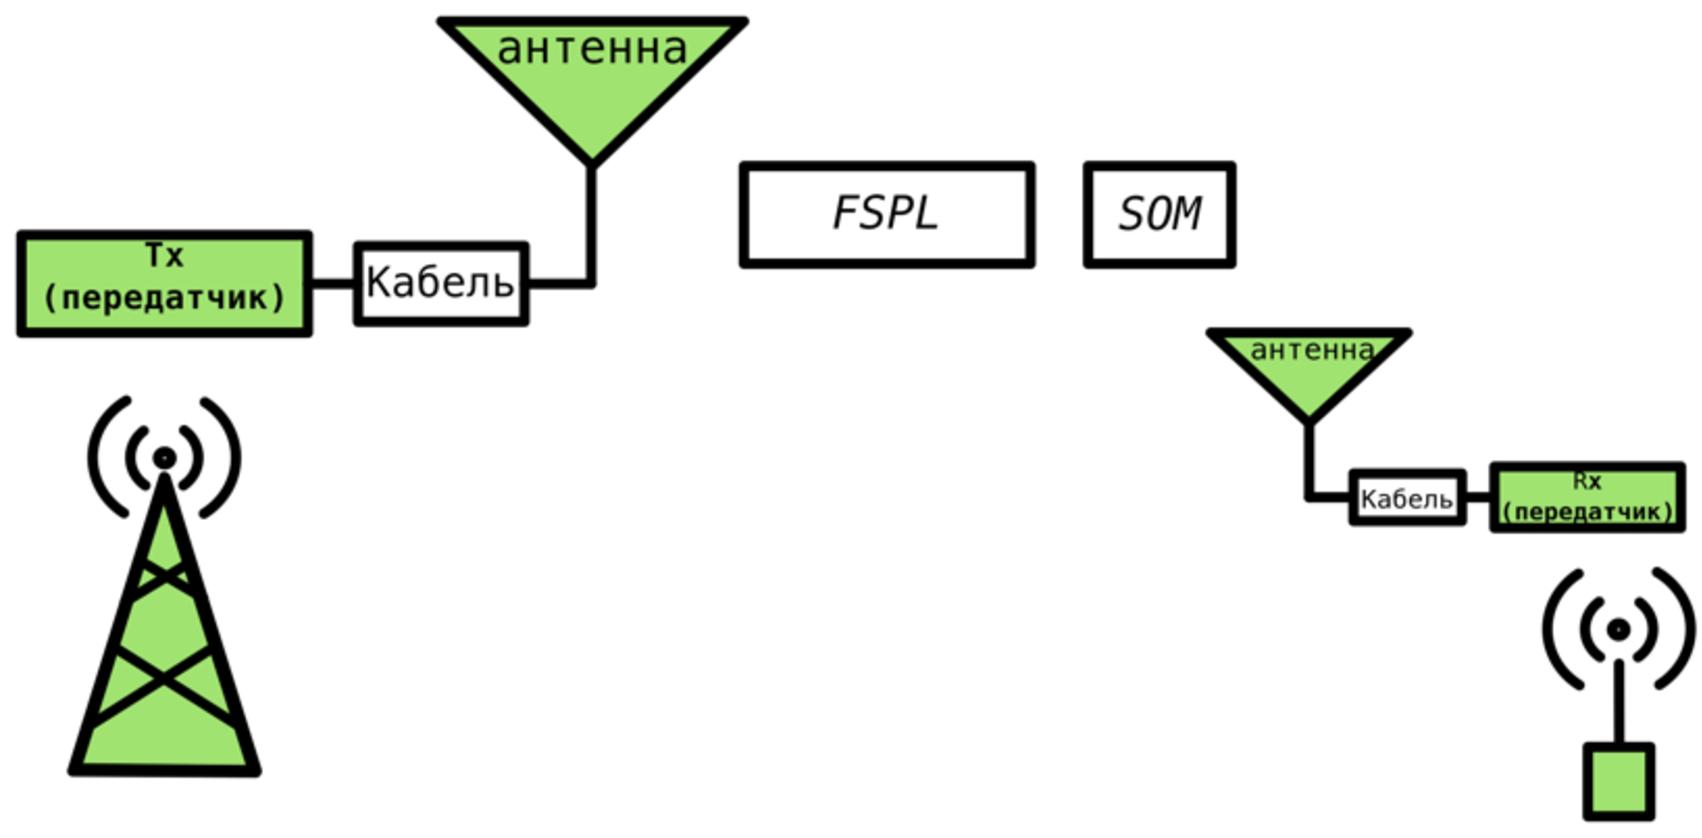
\includegraphics[width=0.8\textwidth]{coverage.pdf}
% \caption{Покрытие станции.}
% \label{fig:part3_coverage}
% \end{figure}
  




\underline{\textbf{Вторая глава}} посвящена задаче оптимального размещения базовых станций БШС для контроля линейной территории. Проблема формулируется в виде задачи ЦЛП и в виде комбинаторной модели в экстремальной форме.

Задаче в виде ЦЛП формулируется следующим образом. 

Для контроля над заданным линейным участком необходимо разместить базовые приемопередающие станции (далее называемые станциями) таким образом, чтобы максимизировать покрытие с ограничениями на суммарную стоимость размещенных станций.

Целевая функция будет представлена как:
$$
  f =  \sum\limits_{i=1}^n (y_i^- + y_i^+) \rightarrow max,
$$
где $y_i^+$ и $y_i^-$ , $i= \overline{0,n+1}$ определяют охват покрытия (справа и слева, соответственно) станций.

Важно обеспечить связь любой станции со шлюзами на концах участка через систему размещенных станций. Задано множество станций $S = \{s_j\}$. Каждой станции приписаны параметры $s_j = \{r_j, \{R_{jq}\}, c_j \}$, $j = \overline{1,m}; q = \overline{1,m}; q \neq j$. Здесь $r_j$ -- радиус покрытия станции, $R_{jq}$ -- это радиус связи между станцями $s_j$ и $s_q$, и $c_j$ -- это стоимость. Задан линейный участок длиной $L$ с концами в точка $a_0$ и $a_{n+1}$. Внутри  отрезка $[a_0, a_{n+1}]$ задано конечное множество точек $A=\{a_i\}, i=\overline{1,n}$; эти точки соответствуют набору свободных мест, где могут быть размещены станции. Каждая точка $a_i$ определяется своей одномерной координатой $l_i$. Заданы станции специального вида $s_{m+1}$ -- шлюзы. Данные шлюзы размещены на концах $a_0$ и $a_{n+1}$ данного линейного участка. Для данных станций параметр радиуса покрытия $r_{m+1}=0$. Радиус связи и стоимость не заданы.


Была получена математическая модель в виде задачи целлочисленного-линейного программирования. Для частного случая, представленного в работе \cite{Ivanov2018}, где размещаются множество однотипных станций вдоль линейного участка, представлено докозательнство NP-полноты. Данная модель является обощением частного случая, следовательно также является NP-полной. Модель ЦЛП рассчитывалась алгоритмом Лэнд и Дойг \cite{Land1960}. 

Одной из важных характеристик производительности сети является ее межконцевая задержка. Необходимо оценивать характеристику и использовать ее в качестве ограничения при синтезе топологической структуры сети К сожалению, представить данное ограничение в линейной форме невозможно. 

Для удовлетворения данного ограничения в главе представлена постановка задачи и ее формулировка в экстремальной комбинаторной форме.

\textit{Допустимой расстановкой станций} назовем такой возрастающий по величине координат $l_i$  набор пар $P = \{a_i, s_j\},a_i \in A,i \neq 0,i \neq n+1;s_j \in S$, для которого выполняются требования:

\begin{enumerate}
    \item  для каждой пары $(a_i,s_j)$:
        \begin{enumerate}
            \item слева: либо найдется такая пара $(a_k,s_q)$, что, $l_i - l_k \leqslant R_{jq}$  и $l_i - l_k  \leqslant R_{qj}$, либо $l_i-l_0 \leqslant R_{j0}$ и $l_i - l_0 \leqslant R_{0j}$;
            \item справа: либо найдется такая пара $(a_t,s_g)$, что, $l_t-l_i \leqslant R_{jq}$ и $l_t - l_i \leqslant R_{qj}$, либо $l_{n+1}-l_i \leqslant R_{j(m+1)}$ и $l_{n+1}-l_i \leqslant R_{(m+1)j}$. 
        \end{enumerate}

Данное требование гарантирует, что любая станция может быть связана со станциями на концах отрезка либо через промежуточные станции, либо непосредственно;
    \item в одной точке стоит не более одной станции;
    \item сумма задержек по всем размещенным станциям меньше заданной величины $T$ – средней межконцевой задержки по времени по всей системе станций:
    \begin{displaymath}
        \label{eq:part3_e2e_delay}
        \sum\limits_{j \in S_\sigma} \overline{T_j} \leqslant T,
    \end{displaymath}
где $S_\sigma$ – множество размещенных станций, $\overline{T_j}$ -- среднее время задержки на станции. Расчет задержек описан в параграфе \cref{part4_e2e_delay_section}
    \item суммарная стоимость размещенных станций меньше заданного бюджетного ограничения  $C$.
\end{enumerate}

Каждой допустимой расстановке станций $P$ соответствует величина покрытия $z(P)$, определяемая как суммарная область покрытия станции, входящих в набор пар $P$.

Для удобства описании в дальнейшем алгоритмов введем понятие «недопокрытия»:

\begin{displaymath}
    f(P) = L - z(P)
\end{displaymath} 

\textbf{Задача 1.}
Пусть $G$ -- множество всех допустимых расстановок $P$.
Тогда требуется найти такую допустимую расстановку  $P^*$, что
\begin{equation}
    \label{eq:part3_P}
    P^* = \argmin \limits_{P \in G} f(P)
\end{equation}

Обозначим через $\Gamma$ все множество вариантов размещения станций (не обязательно допустимых) из множества $S$ на заданном множестве возможных мест их размещения.


Обозначим через $\Gamma$ все множество вариантов размещения станций (не обязательно допустимых) из множества $S$ на заданном множестве возможных мест их размещения. В множестве $S$ станции упорядочены по не убыванию радиусов покрытия. 
Описываемая процедура использует известный прием разбиения множества $G$ на подмножества с использованием некоторого параметра. Процесс формирования и последовательность исследования подмножеств обычно представляется с помощью дерева поиска, представляющего собой ориентированное от корня «дерева ветвлений», где каждому подмножеству соответствует вершина на дереве. Множеству $\Gamma$ соответствует корневая вершина.

В главе предствлена процедура построения бинарного дерева поиска (дерева ветвлений) для полного перебора без повторений всех элементов множества $\Gamma$. Данная процедура будет использована в дальнейшем при построении дерева поиска в алгоритме МВиГ


Пусть $G_0$, где нижний индекс – номер итерации, исходное множество $\Gamma$. На каждой итерации, начиная с итерации $\nu=0$, разбиваем текущее подмножество $G_\nu$ на два подмножества $G^1_\nu$ и $G^2_\nu$. При этом множество $G_\nu$ обычно называется «материнским», а множества $G^1_\nu$  и $G^2_\nu$  - «потомками» множества $G_\nu$ или дочерними узлами.

В качестве параметра разбиения воспользуемся переменной $\pi_{ij}$, принимающей два значения 0 и 1:

\begin{itemize}
    \item $\pi_{ij}=1$, если наложено условие, что на месте $a_i$ расположена станция $s_j$;
    \item $\pi_{ij} = 0$, если наложено условие, что на месте $a_i$ станция $s_j$  располагаться не будет.
\end{itemize}

Алгоритм метода ветвей и границ.

Для построения алгоритма МВиГ были разработаны методы исследования вершин дерева на возможность их закрытия.
В соответствии с техникой МВиГ закрытие вершины в результате исследования, соответствующего ей множества $G_\nu$ возможно в трех случаях.

\underline{\textit{\textbf{Случай 1.}}} Множество $G_\nu$ -- пусто, т.е. доказано, что в множестве $G_\nu$ при данном наборе фиксированных и запрещенных переменных $\pi_{ij}$ нет ни одной допустимой расстановки $P$.

\underline{\textit{\textbf{Случай 2.}}} Доказано, что в множестве $G_\nu$ не может быть допустимой расстановки P с меньшим значением целевой функции (1), чем у лучшей расстановки $\widehat{P}$ из уже найденных. Значение функции $f(\widehat{P})$ называется «рекордом», а расстановка $\widehat{P}$ -- «рекордным решением». В качестве начального рекорда принимается число заведомо большое искомого оптимального решения, например, $L$ – длина всего отрезка.

\underline{\textit{\textbf{Случай 3.}}} Найдено оптимальное решение на множестве $G_\nu$.
% Прежде чем рассмотреть эти три случая, запишем важное свойство любого множеств $G_\nu$, являющееся следствием принятого правила выбора свободной переменной для разбиения очередного множества $G_\nu$ при прямом шаге.

На каждом узле проводится оценка "недопокрытия"  в виде суммы

\begin{displaymath}
    W\left(G_\nu\right) = w_1 + w_2. 
\end{displaymath}

Величина $w_1 \left(G_\nu \right)$ вычисляется как сумма все частичных «недопокрытий» слева от точки размещения $a_k$ и величины радиуса покрытия, размещаемой станций. Оценку $w_2 \left(G_\nu \right)$ вычисляется «для недопокрытия» справа на части $\beta$ до конца всего отрезка (точки $a_{n+1}$). Данную оценку получим релаксацией условий, определяющих допустимую расстановку станций на участке $\beta$. Найдем такое подмножество $S_\beta$ множества станций $S$, состоящее из еще не размещенных станций и дающее минимальное «недопокрытие» на участке $\beta$ при выполнении только условий 2) – 4). Для этого сформулируем следующую задачу булевого программирования.

\underline{\textit{\textbf{Задача 2.}}}
\begin{displaymath}
    z = |\beta| - \sum\limits_{x_j \in S_\beta} r_j x_j \rightarrow min.
\end{displaymath}
при условии:

\begin{equation}\label{eq:part4_task2_cost}
    \sum\limits_{x_j \in S_\beta} c_j x_j \leqslant C,
\end{equation}

\begin{equation}\label{eq:part4_task2_m}
    \sum\limits_{x_j \in S_\beta} x_j \leqslant m,
\end{equation}

\begin{displaymath}
    x_j \in \{0, 1\},
\end{displaymath}
где $|\beta|$ -- длина отрезка отрезка  $\beta$, $m$ -- число свободных мест для размещения станций на отрезке $\beta$.

Очевидно, что эффективность использования оценки в методе ветвей и границ определяется точностью оценки и временем ее вычисления. \underline{\textit{\textbf{Задача 2}}} -- это задача ЦЛП, являющаяся труднорешаемой \cite{Gari}. На основании \underline{\textit{\textbf{задачи 2}}} можно получить две оценки менее точные, но имеющие более эффективные методы решения. Заметим, что при снятии ограничения \cref{eq:part4_task2_cost} или \cref{eq:part4_task2_m} \underline{\textit{\textbf{задача 2}}} представляет собой целочисленную задачу о ранце c эффективным псевдополиномиальным алгоритмом решения \cite{Gari}. При этом с точки зрения точности оценки, более перспективным представляется снятие ограничения \cref{eq:part4_task2_m}, так как на практике, обычно, число возможных мест размещения станций существенно меньше числа размещенных станций, полученного в результате решения задачи. 

Если множество $G_\nu$ получено из материнского добавлением условия $\pi_{kt}=0$, то оценка $W(G_\nu)$ равна оценке материнского множества.

Если для найденной расстановки $P$ выполняются условия 1) – 4), которые для единственной расстановки легко проверяются, и

\begin{equation}
    \label{eq:part4_is_less_than_record}
    f(P) < f(\widehat{P}),
\end{equation}
то $f(P)$ принимается за новый рекорд $f(\widehat{P})$, расстановка $P$ становиться новым рекордным решением $\widehat{P}$ и выполняется шаг обратного хода по дереву поиска. Если неравенство \cref{eq:part4_is_less_than_record} не выполняется, то рекорд остается прежним и выполняется шаг обратного хода.

Работа алгоритма МВиГ заканчивается, когда все вершины дерева поиска закрыты, при этом решение задачи: 

\begin{displaymath}
    P^{*} = \widehat{P},  f(P^*) = f(\widehat{P}).
\end{displaymath}

Был проведено численное сравнение двух моделей для частного случая с однотипными станциями и без учета ограничения на время доставки пакетов в сети. В задаче требовалось разместить весь набор $m$ имеющихся станций. Множество всех возможных вариантов комбинаций $m$ станций на  $n$ местах (не только допустимых) запишем как $\Gamma$. Общее количество $\gamma \in \Gamma$:

\begin{displaymath}
\gamma = C_n^m \times m!.
\end{displaymath} 
 
В качестве характеристики сравенения двух методов было выбрано количество пройденных узлов в ходе поиска оптимального значения, чтобы параметры выполнения алгоритмов не зависели от скорости машины и/или качества реализации программного кода данных алгоритмов.

В таблице \cref{tab:problems_BF_BnB_ILP} показаны результаты решения задач для различного числа количества размещения и количества станций с использованием полного перебора, алгоритма МВиГ и модели ЦЛП. Для каждого набора станций и набора размещений были рассчитаны 10 примеров с различными числовыми входными данными. Для <<$-$>> решение задачи данной размерности методом полного перебора не было получено за 3 ч счета. 
Как видно из результов, представленных в таблице, при увеличении размерностей задачи, алгоритм МВиГ позволяет найти решение быстрее в ходе движения по дереву поиска.

\begin{table}[b]\centering
    \caption{Результаты численного решения.}\label{tab:problems_BF_BnB_ILP}
    \begin{tabular}{|l|l|l|l|l|}
    \hline
    \textbf{Места размещения} & \textbf{Станции} &	\textbf{Полный перебор}& \textbf{МВиГ} & \textbf{ЦЛП} \\ 
    \hline
    7 &		5 &	17550  &	933 &		753\\
    9 &		5 &	71090  &	6478 &		2669\\
    10 &	5 &	126180 &	1041 &		8551\\
    12 &	6 &	-- &		8294 &		38569\\
    13 & 	6 &	-- &		18485 &		30369\\
    \hline
    \end{tabular}
\end{table}
    

\textbf{Построения последовательности топологий для итерационной процедуры моделирования.}

При проектировании БШС надо найти ее оптимальную топологию среди всех топологий, для которых будут выполняться все требования к показателям, исследуемым и рассчитываемым на этапе моделировании сети. Для решения этой задачи воспользуемся идеей метода построения последовательности планов \cite{Emelichev}.

Рассмотрим \textbf{задачу 1.}

Требуется найти такую допустимую расстановку $P^*$, что

\begin{displaymath}
    f(P^*) = min \{f(P), P \in G \}.
\end{displaymath}

Построим для этой задачи последовательность $\Gamma = P^1, P^2, ... ,P^k$ допустимых расстановок (решений) множества $G$ для заданного $k$, где 
\begin{align}
    f(P^1) &= f(P^*), \nonumber  \\
    f(P^2) &= extr\{ f(P), P \in G \ P^1 \}, \nonumber \\
    ... \nonumber \\
    f(P^k) &= extr\{ f(P), P \in G \ P^1 \cup P^2 \cup ... P^k \}, \nonumber 
\end{align}

В последовательности $\Gamma$ каждое решение не лучше предыдущего и не хуже последующего.

Будем последовательно, начиная с первой расстановки, выполнять этап моделирования БШС. Очевидно, что как только мы получим расстановку, удовлетворяющую всем требованиям этапа моделирования, мы решим задачу нахождения оптимальной топологии среди всех топологий, для которых выполняются все требования к показателям, исследуемым и рассчитываемым на этапе моделировании сети. Действительно, для всех предыдущих расстановок эти условия не выполняются, а все последующие расстановки в последовательности $\Gamma$ не могут быть лучше по критерию $f(P)$.

Заменив неравенство \cref{eq:part4_is_less_than_record} на нестрогое и записывая все рекорды, полученные в процессе работы алгоритма, мы, очевидно, получим последовательность расстановок, где каждая расстановка не хуже предыдущей и не лучше последующей. Для получения последовательности $\Gamma$ достаточно «перевернуть» полученную последовательность, где первый элемент станет последним.

Недостатком такой процедуры является то, что для исследования на этапе моделирования будут отобраны только расстановки не хуже первого рекорда и среди них может не оказаться расстановки, удовлетворяющей критериям моделирования.
Для расширения множества $\Gamma$ можно сделать следующее. Зададим условие. что в результате решения \textbf{задачи 1} мы хотим получить не только оптимальное решение, но и все решения не хуже оптимального на величину $d$. Для решения такого варианта задачи достаточно неравенство \cref{eq:part4_is_less_than_record} в алгоритме \fixme{МВиГ} заменить следующим неравенством 

\begin{equation}
    \label{eq:part4_is_less_than_record_d}
    f(P) \leqslant f(\widehat{P}) + d,
\end{equation}
где $d = \varepsilon \cdot L > 0, \varepsilon$ -- заданное отклонение в процентах, и запоминать все рекорды, полученные в процессе решения задачи.

На основании неравенства \cref{eq:part4_is_less_than_record_d} можно построить итерационную процедуру, увеличивая величину $d$, если при данном ее значении допустимого решения на этапе моделирования не найдено.

Обе задачи, в виде ЦЛП и в виде комбинаторной модели в экстремальной форме относятся к широкому к классу задач размещения мощностей. Отличительной особенностью рассмотренных задач является наличие условия связи между станциями.

\underline{\textbf{Третья глава}} посвящена исследованию оптимальное размещение базовых станций БШС связи для обслуживания заданного множества рассредоточенных объектов. Данный случай является обобщением задачи покрытия линейного участка. Специфика данной задачи размещения мощностей также является наличия условия связи между станциями.

Постановка задачи

Задано множество вершин $A = a_i$, $i=\overline{0,n}$ на плоскости. Каждая вершина $a_i$ имеет координаты $\left\{ x_i, y_i \right\}$.
Множество $A$ состоит из двух подмножеств: 
\begin{itemize}
    \item $A_1$ -- множество вершин, с которых необходимо собирать информацию. Каждой вершине $a_i$ приписана   величина $v_i$ -- максимальный объем информации, снимаемой с объекта, расположенного на этой вершине;
    \item $A_2$ -- множество возможных мест размещения базовых станций. 
\end{itemize}

По определению

$$
A_1 \cup A_2 = \varnothing;
$$

$$
A_1 \cap A_2 = A.
$$

Все вершины пронумерованы так, что $
A_1 = \left\{a_i \right\}, i= \overline{1,n_1};
$ и $
A_2 = \left\{ a_i  \right\}, i= \overline{n_1+1,n}.
$


Задано множество типов базовых станций $S = s_j$, $j=\overline{1,s}$, которые необходимо разместить на множестве $A_2$. Каждой станции приписаны четыре параметра $s_j = \left\{r_j, R_j, \vartheta_j, c_j \right\}$, где:
$r_j$ -- максимальный радиус покрытия; $R_{ij}$ -- максимальный радиус связи между $i$-ой и $j$-ой станциями. Параметр характеризует расстояние, на котором обеспечивается связь между станциями; $\vartheta_j$ -- максимальный объем информации в единицу времени, который может быть получен от объектов, обслуживаемых данной станцией; $c_j$ -- стоимость станции.

% \begin{itemize}
%     \item $r_j$ -- максимальный радиус покрытия;
%     \item $R_{ij}$ -- максимальный радиус связи между $i$-ой и $j$-ой станциями. Параметр характеризует расстояние, на котором обеспечивается связь между станциями;
%     \item $\vartheta_j$ -- максимальный объем информации в единицу времени, который может быть получен от объектов, обслуживаемых данной станцией;
%     \item $c_j$ -- стоимость станции.
% \end{itemize}

% Также задана станция специального вида (шлюз) $s_0 = \left\{ r_0, R_0, \vartheta_0, c_0 \right\}$ с координатами $\left\{x_0, y_0 \right\}$, где $r_0 = R_0 = \vartheta_0 = c_0 = 0$


Требуется разместить станции таким образом, чтобы вся информация с объектов (вершинах множества $A_1$) могла быть собрана и передана системой станций, размещенных на выбранных в результате решения задачи вершинах множества  $A_2$, до шлюза $s_0$ и общая стоимость размещенных станций была бы минимальной.
Вершины и станции будем, соответственно, идентифицировать как объекты или станции на них размещенные.
Задано условие, что информация c вершин множества $A_1$ может передаваться непосредственно только на вершины множества $A_2$, а со шлюзом и между собой могут быть связаны только вершины множества $A_2$.

% \fixme{Заметим, что в отличие от предыдущих двух задач в данной задаче задано не множество станций, которые все должны быть использованы в проектируемой сети, а только типы станций. Таким образом в результате решения задачи определяется как набор станций, так и места их размещения.}
% Формулировка задачи в виде модели частично целочисленного ЛП.
Задано $m$ типов станций. Вместо каждой вершины $ai$, $i= \overline{n_1+1,n}$ введем $m$ вершин с координатами вершины $a_i$, и различными параметрами, соответствующими различным типам станций. Обозначим такую группу вершин, записанных с одинаковыми координатами вместо вершины $a_i$,как $D_i$. Каждой вершине из $D_i$ поставим в соответствие набор параметров только одного типа станции из $S$, т.е. на данной вершине может стоять либо станция приписанного типа либо никакая. Обозначим расширенное множество вершин $A_2$ через $A_2D$.

Составим граф $H=\left\{AD,E\right\}$, описывающий сеть для передачи потока информации между вершинами расширенного множествa $AD=A_1 \cup A_2D$ и шлюзом.
Матрица смежности $E = e_{ij}$ графа $H$ строится по следующим правилам.

\begin{itemize}
    \item $e_{ij} = 1$, если расстояние между $i$-ой вершиной ($a_i \in A_1$) и $j$-ой вершиной ($a_j \in A_2D$) не более радиуса покрытия, приписанного этой вершине;
    \item $e_{ij} = 1$, если вершины $a_i$ и $a_j$   принадлежат разным множествам $D_i$ и $D_j$ и расстояние между ними не более радиуса связи той вершины, у которой радиус связи не больше радиуса связи другой вершины;
    \item $e_{i0} = 1$ ($a_i \in A_2D$ ) если расстояние от вершины до шлюза не более $R_i$;
    \item $e_{ij} = 0$, во всех остальных случаях.
\end{itemize}

% Введем потоковые переменные $x_{ij} \geqslant 0$.

% Распишем условия для нашей задачи.
% Величина суммарного потока, который выходит с вершины $a_i$ равен весу $\vartheta_i$

% \begin{equation}\label{eq:part2_1.5}
%     \sum_{a_j \in \Gamma^+(a_i)} x_{ij} = \vartheta_i, \forall a_i, i =\overline{1, n_1};
% \end{equation} 
% где $\Gamma^+(a_i)$ -- множество вершин на графе $H$, в которые входят дуги, исходящие из вершины $a_i$.

% Сумма входящих и выходящих потоков для любой $i$-ой вершины множества $A_2D$ равна нулю
% \begin{equation}\label{eq:part2_1.6}
%     \sum_{a_j \in \Gamma_1^-(a_i)} x_{ij} + \sum_{a_j \in \Gamma_2^-(a_i)} x_{ji} -  \sum_{a_j \in \Gamma_2^+(a_i)} x_{ij} =0 ,\forall a_i \in A_2. 
% \end{equation} 

% Здесь множество $\Gamma_1^-(a_i)$ -- вершины множества $A_1$, из которые выходят дуги, входящие в вершину $a_i$, $\Gamma_2^-(a_i)$ -- вершины множества $A_2D$, из которых выходят дуги, входящие в  вершину $a_i$, $\Gamma_2^+(a_i)$ -- вершины множества $A_2D$, в которые входят дуги, исходящие из вершины  $a_i$.

% Через систему станций вся информация от объектов  должна поступить на шлюз $s_0$ 

% \begin{equation}\label{eq:part2_1.7}
%     \sum_{a_j \in \Gamma_2^-(a_0)} x_{j0} = \sum_{a_i \in A_1} \vartheta_i.
% \end{equation}
% Здесь $\Gamma_2^-(a_0)$ –- подмножество вершин множества $A_2D$, дуги которых входят в шлюз $a_0$.

% Введем булевы переменные $y_i$ для вершин $a_i$, $ai \in A_2D$
% \begin{itemize}
%     \item $y_i = 1$, если станция стоит на месте $a_i$;
%     \item $y_i = 0$, в противном случае.
% \end{itemize}

% Объем информации, поступающей от вершин множества $A_1$ на вершину $a_i \in A_2D$, ограничен мощностью станции $\vartheta_i$.

% \begin{equation}\label{eq:part2_1.8}
%     \sum_{a_j \in \Gamma^-(a_i)} x_{ji} \leqslant y_i \cdot \vartheta_i, \forall a_i \in A_2D.
% \end{equation}

% На множестве $D_i$ может быть размещено не более одной станции 


% \begin{equation}\label{eq:part2_1.9}
%     \sum_{a_j \in D_i} y_j \leqslant 1, \forall D_i.
% \end{equation}

Целевая функция задачу минимазции суммарной стоимости:

$$
    \sum_{a_i \in A_2D} c_i \cdot y_i \to min,
$$
где $y_i = 1$, если станция стоит на месте $a_i$ и $y_i = 0$, в противном случае.

% Задача \cref{eq:part2_1.5, eq:part2_1.6, eq:part2_1.7, eq:part2_1.8, eq:part2_1.9, eq:part2_1.10} представляет собой частично целочисленную задачу линейного программирования с $s \cdot |A_2|$ булевыми переменными.


% Можно сослаться на свои работы в автореферате. Для этого в файле
% \verb!Synopsis/setup.tex! необходимо присвоить положительное значение
% счётчику \verb!\setcounter{usefootcite}{1}!. В таком случае ссылки на
% работы других авторов будут подстрочными.
% Изложенные в третьей главе результаты опубликованы в~\cite{vakbib1, vakbib2}.
% Использование подстрочных ссылок внутри таблиц может вызывать проблемы.

В \underline{\textbf{четвертой главе}} приведено описание метода оценки времени межконцевой задержки сети для случая с зависимым временем осблуживания на фазах.

Одним из важных ограничений для алгоритма МВиГ является межконцевая задержка сети. В класическом случае для расчета межконцевой задержки сети рассмотривают простейшую модель многафазной сети массового обслуживания  с узлами $M/M/1$ c линейной топологией и $N$ последовательно соединенными узлами. В такой системе время между поступлениями новых пакетов и время из обслуживания на каждой фазе принадлежат экспоненциальному закону распределения. Интервал между поступлениями пакетов задается случайной величиной $A \sim Exp(\lambda)$. Время обслуживания в такой системе задается непосредственно, с помощью случайной величины $S \sim Exp(\mu)$. Для такого простейшего случая имеется аналитическое решение. По теореме Литтла легко рассчитать среднее время пребывание пакетов на каждом узле. Межконцевая задержка в итоге будет суммой всех задержек на каждой фазе сети. Аппарат теории массового обслуживания описывает систему с марковским случайным процессом, одним из допущеннии которых является допущение о независимости обслуживания. Другими словами обслуживание пакетов на каждом узле происходит случайно и независимо от других узлов.  
В реальности же, пакеты, появившись в беспроводной сети не изменяют своего размера в течение всего времени обслуживания на всех фазах, а значит и время его обслуживания будет постоянным на всех последующих фазах. Так как нам интереснее рассматривать размеры пакетов, то вместо случайной величины $S$, определяющей время обслуживания, мы будем задавать в виде случайной величины размер пакетов в битах $C \sim Exp(\gamma)$, а время передачи определять как $T_n = C/R_n$, где $R_n = \frac{\mu}{\gamma}$ - битовая скорость передачи, задаваемая константой.

Если размер пакета определяется случайно каждый раз, когда начинается его обслуживание, то такая сеть массового обслуживания оказывается классической сетью с узлами $M/M/1$. Если же размер пакета определяется при его поступлении в сеть и далее не изменяется, то между обслуживаниями одного пакета на разных узлах появляется связь. 
Для оценки времени межконцевой задержки с зависимым обслуживанием аналитических решений не существует. Для проверки предположения влияния фиксации размеров пакетов при их первом появлении (зависимости обслуживании) построим имитациионную модель, в которой методом Монте-Карло разыграем несколько сотен тысяч пакетов для расчете среднего времени задержек в системе. Имитационную модель построим для сети с количеством узлов $N=20$. По данным на выходе модели построим графики задержек и длин очередей на фазах от коэффициента загрузки. Сравним полученные результаты с аналитическим решением. На рисунке \cref{fig:sim20_model} представлены средние задержки на фазах в зависимости от коэфициентов загрузок $\rho = \{0.3, 0.5, 0.65, 0.8, 0.9\}$. Сплошной линией -- данные имитационной модели с зависимым распределением времения обслуживания, пунктирной -- аналитическое решение. Пурпурным цветом представлены длины очередей на фазах при зависимом времени, голубым цветом представлено аналитическое решение. По резульатом экспериментом можно сделать вывод о влияни факта фиксирования длины пакетов, т.е. с зависимом распределением времени обслуживания. Так как аналитического решения для сети массового обслуживания с зависимым распределением времени обслуживания не существует, единственным возможным вариантов оценки времени межконцевой задержки остается использование имитационного моделирования. Такой подход обладает одним существенным недостатком, а именно большие трудозатраты по времени. Метод Монте-Карло требует генерации несколько сотен тысяч пакетов. При проверке ограничения с помощью имитационного моделирования, в ходе движение по дереву поиска в алогритме МВиГ, тратится большое количество расчетного времени, что делает практически невозможным поиск оптимального решения за адекватное время. Решением данной проблемы будет аппроксимация данных имитационного моделирования с помощью методов машинного обучения (МО).

\begin{figure}[h!]
    \centering
     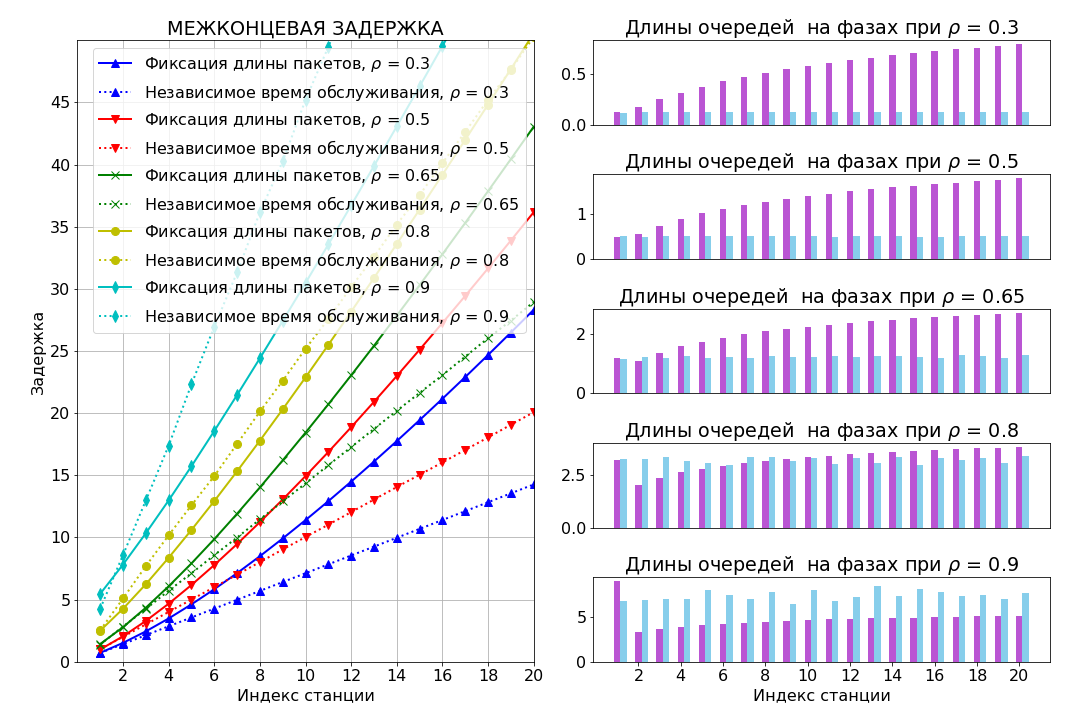
\includegraphics[width=0.8\textwidth]{sim20_model.png}
  \caption{Задержки для случаев с независимой и зависимой функции распределения времени обслуживания}
  \label{fig:sim20_model}
\end{figure}

На вход имитационной модели подавались:
\begin{itemize}
    \item $N$ -- число станций в сети;
    \item $M$ -- размер буфера очередей на фазах;
    \item $m_A$ -- cреднее значение случайного времени между поступлениями пакетов;
    \item $\sigma_A$ -- стандартное отклонение случайного времени между поступлениями пакетов;
    \item $R$ -- битовая скорость;
    \item $m_C$ -- cреднее значение случайного размера пакетов;
    \item $\sigma_C$ -- стандартное отклонение случайного пакетов;
\end{itemize}

Средние значения (или математеское ожидание) и стандартные отклонения случайных величин были взяты с реальных данных. По этим параметрам проводилась апроксимация случайных величин. Если коэффициент вариации $c_v = \frac{\sigma}{m} < 1$, то распределение принадлежит распределения Эрланга. Если $c_v =1$, то экспоненциальному закону. Если $c_v > 1$, то случайная величина принадлежит гиперэкспоненциальное распределению. 

На выходе рассчитывалась межконцевая задержка сети $\overline{T}$. Было сгенирована выборка объемом 80000 строчек. Методом Монте-Карло для каждого случая прогонялись 100000 пакетов. Полученные данные использовались для обучения регрессионных моделей методомами МО. Регрессионные модели строились с помощью метода наименьших квадратов, с помощью дерева принятия решения \cite{Gordon1984}, градиентного бустинга \cite{Friedman2002}, и искусственные нейронные сети на алгоримет Адам \cite{Kingma2015}. На рисунке \cref{fig:total_scatter_diagram} представлены диаграммы рассеивания на тестовой выборке полученных регресиионных моделей. Наименьшим разбросом данных обладает регресионная модель, построенная на алгоритме Адама. Исходя из полученных результатов можно сделать вывод о целесообразности использования модели искусственной нейронной сети для оценки времени межконцевой задержки.


\begin{figure}[h!]
    \centering
     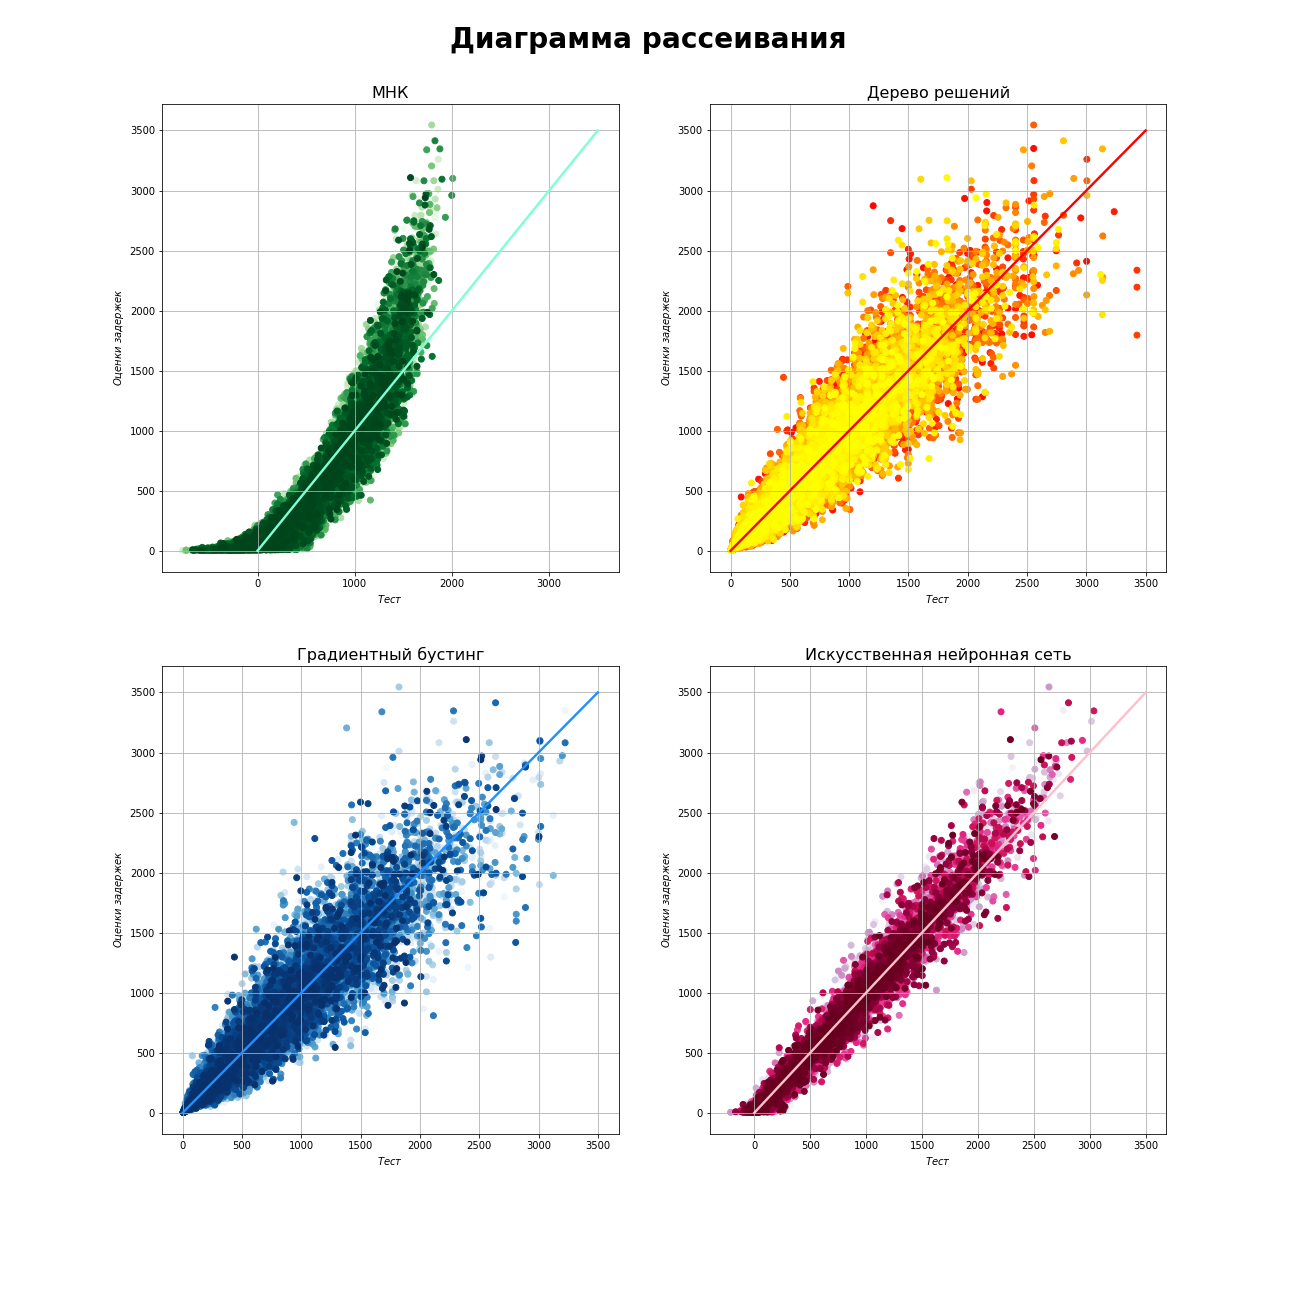
\includegraphics[width=0.86\textwidth]{total_scatter_diagram.png}
  \caption{Диаграмма рассеивания полученных моделей}
  \label{fig:total_scatter_diagram}
\end{figure}

\begin{table}[b]\label{tab:total_reg_metrics}
    \caption{ Метрики моделей}
    \begin{tabular}{|c|ccc|}
        \toprule
        Регрессионные модели    &$R$    & $STD$    &   $MAPE$\\
    
        \midrule
        \textbf{Метод наименьших квадратов} & 0,93   &   210,47  &   23,02 \\
        \textbf{Дерево решений} & 0.95   &   161,19  &   2,14 \\
        \textbf{Градиентный бустинг} & 0.952   &   165,04  &   2,16  \\
        \textbf{Искусственные нейронные сети} & 0.998   &   83,59  &   3,14  \\
        \bottomrule
    \end{tabular}
\end{table}



В таблице \cref{tab:calculation_times} представлены время расчета новой выборки объемом 360. Как видно из расчетов, модели позволяют выиграть время в несколько порядков, что позволяет использовать их в ходе поиска размещения в алгоритме МВиГ.

\begin{table}
    \caption{\label{tab:calculation_times} Оценка времени расчета моделей межконцевой задержки.}
    \begin{tabular}{|cc|}
        \toprule
        \textbf{Модель} & \textbf{Расчетное время, сек} \\
        \toprule
        Имитационная Модель & 172.2 \\
        МНК & $4.77\cdot 10^{-6}$  \\
        Деревья Решений & $5.48\cdot 10^{-6}$ \\
        Градиентный Бустинг & $5.01\cdot 10^{-6}$  \\
        Искусственные Нейронные Сети & $5.72\cdot 10^{-6}$ \\


        \bottomrule
    \end{tabular}
\end{table}


% \begin{table}[H]
%     \caption{\label{tab:total_reg_metrics} Obtained regression models metrics.}
%     \begin{tabular}{cccc}
%         \toprule
%         \textbf{$Model$}    &\textbf{$R$}    & \textbf{$STD$}    &   \textbf{$R^2$}\\
    
%         \midrule
%         \textbf{Least Squares} & 0.926   &   66.309  &   0.857 \\
%         \textbf{Decision Tree} & 0.990   &   24.495  &   0.981 \\
%         \textbf{Gradient Boosting} & 0.990   &   24.714  &   0.980  \\
%         \textbf{Neural Network} & 0.998   &   12.225  &   0.995  \\
%         \bottomrule
%     \end{tabular}
% \end{table}


\FloatBarrier
\pdfbookmark{Заключение}{conclusion}                                  % Закладка pdf
В \underline{\textbf{заключении}} приведены основные результаты работы, которые заключаются в следующем:
%% Согласно ГОСТ Р 7.0.11-2011:
%% 5.3.3 В заключении диссертации излагают итоги выполненного исследования, рекомендации, перспективы дальнейшей разработки темы.
%% 9.2.3 В заключении автореферата диссертации излагают итоги данного исследования, рекомендации и перспективы дальнейшей разработки темы.

\begin{enumerate}
    \item Проведен анализ методики проектирования современных БШС. В рамках такой методики были исследованы проблемы синтеза топологии БШС вдоль протяженных транспортных магистралей: автомобильные дороги, трубопроводные магистрали, лини метрополитена и т.д. 
    \item Предложена новая математическая модель в виде задачи ЦЛП оптимального размещения БС с линейной топологией.
    \item Представлена новая математическая модель задачи оптимального размещения БС в комбинаторной форме. 
    % Данная модель учитывает специфику задачи для нахождения оптимального решения.
    \item Для комбинаторной модели был разработан новый специальный алгоритм типа ветвей и границ. 
    
    % Представлены результаты сравнения поиска оптимального решения с помощью МВиГ с алгоритмами решения задачи в общем виде.
    \item В рамках комплексного проектирования БШС представлена новая итерационная процедура нахождения последовательности лучших решений задачи оптимального размещения БС для случая, когда найденное оптимальное решение построение топологии сети не удовлетворяет некоторым критериями функционирования БШС, проверяемых на следующих этапах проектирования.
    \item Предложена новая математическая модель виде задачи ЧЦЛП оптимального размещения БС для покрытия множества рассредоточенных объектов. 
    \item Разработан программный комплекс для расчета задачи оптимального размещения БС  с помощью предложенного алгоритма типа ветвей и границ.
    \item Представлены результаты численных экспериментов, доказывающие эффективность предложенных моделей и методов для решения задачи синтеза топологии при проектировании БШС.
\end{enumerate}

% \begin{enumerate}
%     \item Был проведен анализ методики проектирования современных БШС. В рамках такой методики были исследованы проблемы синтеза топологии БШС вдоль протяженных участков: трубопроводные магистрали, протяженные автомобильные дороги. 
%     \item Была предложена математическая модель в виде задачи ЦЛП размещения БС с линейной топологией.
%     \item Была представлена математическая модель экстремальной задачи оптимального размещения БС в комбинаторной форме. 
%     % Данная модель учитывает специфику задачи для нахождения оптимального решения.
%     \item Для комбинаторной модели был разработан специальный алгоритм типа ветвей и границ. Представлены результаты сравнения поиска оптимального решения с помощью МВиГ с алгоритмами решения задачи в общем виде.
%     \item В рамках комплексного проектирования была представлена итерационная процедура нахождения последовательности лучших решений задачи оптимального размещения для случая, когда найденное оптимальное решение построение топологии сети не удовлетворяет некоторым критериями функционирования БШС, проверяемых на этапе моделирования процесса передачи данных.
%     \item Предложена математическая модель оптимального размещения БС для покрытия множества рассредоточенных объектов.
%     \item Разработан программный комплекс для расчета задачи оптимального размещения БС  с помощью предложенного алгоритма типа ветвей и границ.
% \end{enumerate}




% \begin{enumerate}
%   \item построены математические модели в виде экстремальной комбинаторной задачи и задачи ЦЛП для оптимального размещения базовых станций при проектировании БШС с линейной топологией;
%   \item представлен алгоритм метода ветвей и границ для задачи размещения базовых станций с линейной топологией; 
%   \item разработана итерационная процедура нахождения последовательности лучших решений для задачи размещения базовых станций в рамках комплексного проектирования БШС с линейной топологией;
%   \item разработаны математические модели для задач проектирования БШС для покрытия множества рассредоточенныз объектов;
%   \item разработаны модели прогнозирования оценок характеристик производительности сети с помощью методов машинного обучения.
% \end{enumerate}


\pdfbookmark{Литература}{bibliography}                                % Закладка pdf
% При использовании пакета \verb!biblatex! список публикаций автора по теме
% диссертации формируется в разделе <<\publications>>\ файла
% \verb!common/characteristic.tex!  при помощи команды \verb!\nocite!

\ifdefmacro{\microtypesetup}{\microtypesetup{protrusion=false}}{} % не рекомендуется применять пакет микротипографики к автоматически генерируемому списку литературы
\urlstyle{rm}                               % ссылки URL обычным шрифтом
\ifnumequal{\value{bibliosel}}{0}{% Встроенная реализация с загрузкой файла через движок bibtex8
    \renewcommand{\bibname}{\large \bibtitleauthor}
    \nocite{*}
    \insertbiblioauthor           % Подключаем Bib-базы
    %\insertbiblioexternal   % !!! bibtex не умеет работать с несколькими библиографиями !!!
}{% Реализация пакетом biblatex через движок biber
    % Цитирования.
    %  * Порядок перечисления определяет порядок в библиографии (только внутри подраздела, если `\insertbiblioauthorgrouped`).
    %  * Если не соблюдать порядок "как для \printbibliography", нумерация в `\insertbiblioauthor` будет кривой.
    %  * Если цитировать каждый источник отдельной командой --- найти некоторые ошибки будет проще.
    %

    %% authorvak
    \nocite{IvanovVAK2019}%
    %
    %% authorwos
    % \nocite{wosbib1}%
    %
    %% authorscopus
    % \nocite{scbib1}%
    \nocite{Ivanov2019}%
    
    \nocite{Mukhtarov2020}%
    %
    %% authorpathent
    % \nocite{patbib1}%
    %
    %% authorprogram
    % \nocite{progbib1}%
    %
    %% authorconf
    \nocite{VishnevskyMukhtarovPershinDCCN2020_RSCI}
    \nocite{LazarevaLarionovMukhtarovITTMM2020_RSCI}
    \nocite{MukhtarovIvanovPershinDCCN2019_RSCI}
    \nocite{MukhtarovPershinVSPU2019_RSCI}
    \nocite{MukhtarovPershinMLSD2019materials_RSCI}
    \nocite{MukhtarovPershinMLSD2019works_RSCI}
    %
    %% authorother
    \nocite{VishnevskyLarionovMukhtarovICAM2020_RSCI}
    \nocite{MukhtarovPershinGUBKIN2019_RSCI}
    \nocite{MukhtarovPershinGUBKIN2018_RSCI}%

    \ifnumgreater{\value{usefootcite}}{0}{
        \begin{refcontext}[labelprefix={}]
            \ifnum \value{bibgrouped}>0
                \insertbiblioauthorgrouped    % Вывод всех работ автора, сгруппированных по источникам
            \else
                \insertbiblioauthor      % Вывод всех работ автора
            \fi
        \end{refcontext}
    }{
        \ifnum \totvalue{citeexternal}>0
            \begin{refcontext}[labelprefix=A]
                \ifnum \value{bibgrouped}>0
                    \insertbiblioauthorgrouped    % Вывод всех работ автора, сгруппированных по источникам
                \else
                    \insertbiblioauthor      % Вывод всех работ автора
                \fi
            \end{refcontext}
        \else
            \ifnum \value{bibgrouped}>0
                \insertbiblioauthorgrouped    % Вывод всех работ автора, сгруппированных по источникам
            \else
                \insertbiblioauthor      % Вывод всех работ автора
            \fi
        \fi
        %  \insertbiblioauthorimportant  % Вывод наиболее значимых работ автора (определяется в файле characteristic во второй section)
        \begin{refcontext}[labelprefix={}]
            \insertbiblioexternal            % Вывод списка литературы, на которую ссылались в тексте автореферата
        \end{refcontext}
        % Невидимый библиографический список для подсчёта количества внешних публикаций
        % Используется, чтобы убрать приставку "А" у работ автора, если в автореферате нет
        % цитирований внешних источников.
        \printbibliography[heading=nobibheading, section=0, env=countexternal, keyword=biblioexternal, resetnumbers=true]%
    }
}
\ifdefmacro{\microtypesetup}{\microtypesetup{protrusion=true}}{}
\urlstyle{tt}                               % возвращаем установки шрифта ссылок URL
